\documentclass[aspectratio=169,11pt]{beamer}

\usetheme{Madrid}
\usecolortheme{default}
\usepackage{lmodern}
\usepackage[utf8]{inputenc}
\usepackage[T1]{fontenc}
\usepackage{amsmath,amssymb}
\usepackage{booktabs}
\usepackage{tikz}
\usetikzlibrary{arrows.meta, positioning}
\usepackage{listings}
\usepackage{xcolor}

\definecolor{manifold}{RGB}{30,90,170}
\setbeamercolor{structure}{fg=manifold}
\setbeamertemplate{navigation symbols}{}
\setbeamertemplate{footline}[frame number]

\title[MANIFOLD]{MANIFOLD}
\subtitle{Un motor matemático para mapear vulnerabilidades}
\author{Proyecto MANIFOLD}
\institute{IR tipada $\cdot$ geometría $\cdot$ topología $\cdot$ verificación formal}
\date{2026}

\begin{document}

\begin{frame}
  \titlepage
\end{frame}

\begin{frame}{El problema: priorizar, no detectar}
  \begin{itemize}
    \item Los SAST clásicos enumeran \emph{patrones}: el cuello de botella real no
          es \emph{detectar} sinks, sino \emph{decidir cuál verificar}.
    \item En OWASP Benchmark~1.2 el índice de Youden $J=\mathrm{TPR}-\mathrm{FPR}$ colapsa:
          SonarQube $J\approx+0.01$, CodeQL $J\approx+0.22$.
    \item \textbf{Pregunta:} ¿puede un campo escalar $V(x)$ sobre el grafo de
          programa priorizar el sink vulnerable?
  \end{itemize}
\end{frame}

\begin{frame}{Experimento principal: oráculo de priorización}
  \begin{center}
  \small
  \begin{tabular}{lcccc}
  \toprule
  Ordenamiento (902 casos vulnerables) & MRR & R@1 & NDCG@5 \\
  \midrule
  DFS (orden de fuente) & 0.848 & 0.755 & 0.882 \\
  taint crudo & \textbf{0.894} & \textbf{0.847} & \textbf{0.916} \\
  $V(x)$ fusionado & 0.872 & 0.805 & 0.899 \\
  aleatorio & $0.709\pm0.042$ & 0.531 & 0.778 \\
  \bottomrule
  \end{tabular}
  \end{center}
  \vspace{1mm}
  \textbf{AUC por señal} (¿predice el sink vulnerable?):
  taint $0.895$ · formal $0.878$ · espectral $0.496$ ·
  topológica $0.500$ · geométrica $\mathbf{0.376}$.
\end{frame}

\begin{frame}{El resultado honesto}
  \begin{itemize}
    \item $V(x)$ \textbf{no} supera al taint crudo: es ligeramente peor ($0.872$ vs.\ $0.894$).
    \item Espectral/topológica: \emph{indistinguibles del azar}; curvatura: \emph{peor que el azar}.
    \item \textbf{Conclusión publicable (negativa):} en OWASP Benchmark los priors
          geométrico y topológico \emph{no sobreviven más allá del taint}.
    \item $\Rightarrow$ El valor de MANIFOLD está en la capa \emph{formal}
          (verificación), no en el prior geométrico. L1/L2/L5: \emph{no soportadas}.
  \end{itemize}
\end{frame}

\begin{frame}{La idea central}
  \begin{center}
  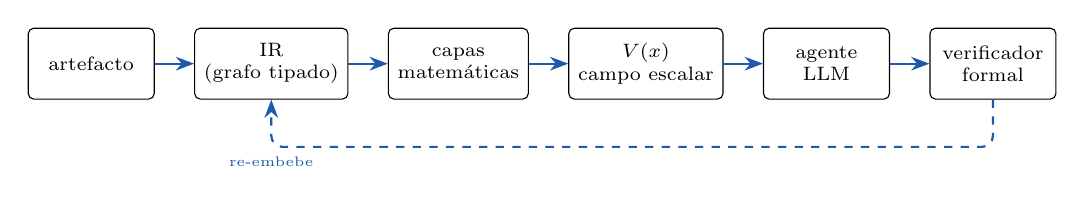
\begin{tikzpicture}[
    node distance=4mm and 5mm,
    box/.style={draw, rounded corners=2pt, minimum height=9mm, minimum width=16mm, align=center, font=\scriptsize},
    arr/.style={-{Stealth}, thick, color=manifold}
  ]
  \node[box] (art) {artefacto};
  \node[box, right=of art] (ir) {IR\\(grafo tipado)};
  \node[box, right=of ir] (layers) {capas\\matemáticas};
  \node[box, right=of layers] (v) {$V(x)$\\campo escalar};
  \node[box, right=of v] (agent) {agente\\LLM};
  \node[box, right=of agent] (verif) {verificador\\formal};
  \draw[arr] (art) -- (ir);
  \draw[arr] (ir) -- (layers);
  \draw[arr] (layers) -- (v);
  \draw[arr] (v) -- (agent);
  \draw[arr] (agent) -- (verif);
  \draw[arr, dashed, rounded corners] (verif.south) -- ++(0,-6mm) -| (ir.south)
    node[pos=0.5, below, font=\tiny]{re-embebe};
  \end{tikzpicture}
  \end{center}
  \begin{itemize}
    \item Una vulnerabilidad \emph{no} es un patrón: es la \emph{violación de una invariante estructural}.
  \end{itemize}
\end{frame}

\begin{frame}{La IR unificada}
  \textbf{Grafo de programa} $G=(V,E,\tau_V,\tau_E,\omega)$:
  \begin{itemize}
    \item \textbf{Nodos}: módulo, función, sentencia, fuente, sumidero, \texttt{gate}, \dots
    \item \textbf{Aristas tipadas}: \texttt{control}, \texttt{data}, \texttt{call}, \texttt{taint}, \texttt{trust}, \texttt{auth}
    \item JSON compartido Python$\leftrightarrow$Rust; agnóstica al artefacto.
  \end{itemize}
  \vspace{2mm}
  \textbf{Multi-dominio}: el \emph{mismo} IR se produce desde
  \begin{itemize}
    \item Python / Java (tree-sitter), binarios (\texttt{objdump} o \texttt{angr}/\texttt{CFGFast}),
    \item OpenAPI (superficie de API), agentes LLM (grafo de herramientas/confianza).
  \end{itemize}
\end{frame}

\begin{frame}{Capas matemáticas}
  \begin{columns}[T]
    \begin{column}{0.5\textwidth}
      \textbf{Espectral} ($L=D-A$)\\
      $\lambda_2$, vector de Fiedler, embedding.
      \vspace{2mm}
      \textbf{Topológica (TDA)}\\
      homología persistente $H_0,H_1$, Mapper.
      \vspace{2mm}
      \textbf{Geométrica}\\
      curvatura de Ollivier--Ricci / Forman--Ricci; Sinkhorn.
    \end{column}
    \begin{column}{0.5\textwidth}
      \textbf{Algebraica}\\
      retículo de taint; naturalidad (categorías).
      \vspace{2mm}
      \textbf{Formal}\\
      ejecución simbólica $+$ SMT (Z3); alcanzabilidad.
      \vspace{2mm}
      \textbf{Dirigida}\\
      Laplaciano de Chung (SCC $+$ Perron).
    \end{column}
  \end{columns}
  \vspace{3mm}
  \begin{center}
  $V(x) = \sigma\!\big(\sum_i \alpha_i\, s_i(x)\big)$ \quad (pesos $\alpha_i$ calibrables)
  \end{center}
\end{frame}

\begin{frame}{Leyes de mapeo (rasgo $\to$ vulnerabilidad)}
  \begin{center}
  \begin{tabular}{cll}
  \toprule
  \# & Rasgo matemático & Clase \\
  \midrule
  L1 & curvatura $\kappa \ll 0$ (cuello de botella) & escalada de privilegios \\
  L2 & generador de $H_1$ persistente & reentrancia / recursión \\
  L3 & corte de Fiedler & inyección cruzando confianza \\
  L4 & flujo de taint que cruza arista \texttt{auth} & violación de naturalidad \\
  L5 & outlier de persistencia & rasgo real vs.\ espurio \\
  L6 & $\mathrm{SAT}(\phi_{\text{malo}})$ & exploit concreto \\
  \bottomrule
  \end{tabular}
  \end{center}
\end{frame}

\begin{frame}[fragile]{El agente neuro-simbólico}
  \begin{enumerate}
    \item \textbf{Mapea}: IR $+$ señales $V(x)$, persistencia, curvatura.
    \item \textbf{Hipotetiza}: el LLM propone sobre regiones priorizadas.
    \item \textbf{Verifica}: Z3 / taint / topología prueba o refuta.
    \item \textbf{Refina} y \textbf{reporta} (witness concreto).
  \end{enumerate}
  \vspace{2mm}
  Reparto de roles: la matemática propone \emph{regiones}; el LLM propone
  \emph{hipótesis}; el solver propone \emph{pruebas}. \\[1mm]
  \textbf{Gramática de verificación}: spec estructurada
  \texttt{(sink, fuente, línea, categoría)} --- el LLM nunca emite SMT-LIB.
\end{frame}

\begin{frame}{Resultados: OWASP Benchmark 1.2}
  \begin{center}
  \small
  \begin{tabular}{lcccccc}
  \toprule
  \textbf{Herramienta} & \textbf{TPR} & \textbf{FPR} & \textbf{Prec.} & \textbf{F1} & \textbf{J} & \textbf{Tiempo} \\
  \midrule
  SonarQube\textsuperscript{(a)} & 0.956 & 0.946 & 0.330 & 0.490 & +0.010 & \textasciitilde3 min \\
  CodeQL\textsuperscript{(a)} & 0.902 & 0.682 & 0.603 & 0.744 & +0.220 & \textasciitilde18 min \\
  \textbf{MANIFOLD} adaptador\textsuperscript{(b)} & 0.842 & 0.674 & 0.572 & 0.681 & \textbf{+0.168} & \textasciitilde45 s \\
  MANIFOLD adaptador $+$ Z3\textsuperscript{(b)} & 0.834 & 0.776 & 0.549 & 0.662 & +0.057 & \textasciitilde4 min \\
  \bottomrule
  \end{tabular}
  \end{center}

  \vspace{1mm}
  {\footnotesize (a) reportado en evaluaciones públicas. (b) \textbf{medido} (Z3 aporta witnesses, no precisión).}
\end{frame}

\begin{frame}{Ablación: de dónde viene la mejora}
  \begin{center}
  \small
  \begin{tabular}{lccc}
  \toprule
  Variante (categorías de taint) & Prec. & Recall & F1 \\
  \midrule
  Adaptador naive inicial & 0.515 & 0.426 & 0.466 \\
  $+$ branch-join, receptor/estado, cobertura & 0.530 & 0.856 & 0.655 \\
  $+$ restricción XSS al writer (final) & \textbf{0.549} & \textbf{0.834} & \textbf{0.662} \\
  \midrule
  final, sin branch-join & 0.515 & 0.555 & 0.535 \\
  \bottomrule
  \end{tabular}
  \end{center}
  \begin{itemize}
    \item \textbf{Branch-join} (supremo del retículo) es la palanca de \emph{recall} ($+0.28$).
    \item La \textbf{restricción del writer HTTP} es la palanca de \emph{precisión}.
    \item Los errores residuales son casos adversariales: los que $V(x)+$Z3 deben recuperar.
  \end{itemize}
\end{frame}

\begin{frame}{Visualización y demo}
  \begin{itemize}
    \item \textbf{Mapa del manifold}: grafo IR con layout force-directed; nodos por tipo,
          aristas por tipo (taint rojo), \texttt{gate} morado.
    \item \textbf{Panel de hallazgos}: \emph{confirmed} (Z3 con witness) vs \emph{candidate}.
    \item \textbf{HTML autocontenido} (sin dependencias) $+$ demo end-to-end sobre 10 artefactos.
  \end{itemize}
  \vspace{2mm}
  \begin{center}
  \texttt{python -m manifold.cli target --agent --viz out.html}
  \end{center}
\end{frame}

\begin{frame}{Conclusiones y trabajo futuro}
  \textbf{Conclusiones}
  \begin{itemize}
    \item Una IR tipada enriquece señales independientes en un campo $V(x)$ navegable.
    \item El reparto neuro-simbólico (matemática/LLM/SMT) es el correcto.
    \item En OWASP Benchmark: $F_1$ $0.466 \to 0.662$ solo con mejoras genéricas de taint.
  \end{itemize}
  \vspace{2mm}
  \textbf{Trabajo futuro}
  \begin{itemize}
    \item Verificación Z3 para Java (cerrar la fila proyectada).
    \item Homología dirigida y Sinkhorn a escala; calibración de $\alpha_i$ sobre corpus reales.
    \item Benchmarks ELF/PE (SARD) sobre el backend binario dual.
  \end{itemize}
\end{frame}

\begin{frame}
  \centering
  \Large\color{manifold}\textbf{Gracias}\\[4mm]
  \normalsize\color{black}
  MAP the code as a space; let geometry reveal the flaw.
\end{frame}

\end{document}
